% !TEX root = ../main.tex

\chapter{Medical information}
\label{ch:medical}
\setlength{\marginparwidth}{3cm}\leavevmode \marginnote{\textbf{Cl{\'e}ment}}This chapter gives an overview of the basic medical knowledge that is required to apprehend the following chapters smoothly. First of all, some notions about cancer are described in order to understand what it is and which effects it has on the human body. Second, medical data has its own file formats. To make use of them in a deep learning project, medical files must be processed in a certain way, depending on each format. In fact, formats represent 2D, 3D or even 4D data. Some of them require specific normalization in order to obtain the right rendering. Finally, some visualization tools that were developed to display raw medical files easily are presented. 


\section{Cancer}
\subsection{Basics}
\setlength{\marginparwidth}{3cm}\leavevmode \marginnote{\textbf{Cl{\'e}ment}}An accumulation of cells forming a mass is called a tumor. These tumors are detectable thanks to medical imaging (see Section \ref{sec:medical_imaging}) and other symptoms. However, not every tumor is as dangerous as the other, as it can be benign (does not contain cancerous cells) or malignant (contains cancerous cells).

The term cancer refers to different phenomena which involve mutation, abnormal multiplication and spreading of cells. As stated by Hanahan et al. in "The Hallmarks of Cancer"~\cite{19} and "The Hallmarks of Cancer: The Next Generation"~\cite{20}, every malignant tumor acquires six different capabilities during its evolution: 
\begin{itemize}
	\item \textbf{"Sustaining proliferative signaling"}\\ Cancerous cells do not wait for the body's approval to grow and proliferate, contrary to normal cells. They become responsible for their own multiplication.
	\item \textbf{"Evading growth suppressors"}\\
The body sends signals to contain cell growth within a tissue. Cancerous cells are insensitive to these. 
	\item \textbf{"Activating invasion and metastasis"}\\
Metastases are cells whose role is to propagate to other parts of the body in order to colonize and create new tumors. 
	\item \textbf{"Enabling replicative immortality"}\\
Healthy cells replication is limited to a certain amount, which is not the case for cancerous cells. 
	\item \textbf{"Inducing angiogenesis"}
\\Angiogenesis is the process of creating new blood vessels. Tumors have an influence on angiogenesis around them, since they need vascularization to continue growing. 
	\item \textbf{"Resisting cell death"}
\\Apoptosis is the programmed death of cells, which is part of the continuous regeneration of every cell within a body. Cancerous cells survive this programmed death. 
\end{itemize}


\subsection{Seriousness}
\setlength{\marginparwidth}{3cm}\leavevmode \marginnote{\textbf{Cl{\'e}ment}}Most cancers can be staged thanks to the TNM system. The T corresponds to the tumor size and its location; the N corresponds to whether or not the tumor has spread to draining lymph nodes; the M corresponds to the presence or absence of metastases in other parts of the body~\cite{21}. These pieces of information are used to classify cancer between four (I to IV) or sometimes five (0 to IV) different stages, reflecting the progression and the seriousness of the illness~\cite{22}. The earlier they are detected, the higher the chances of recovery are. This aspect makes cancer detection critical since every misjudgment can threaten someone's life. 


\section{Types of medical imaging}
\label{sec:medical_imaging}
\setlength{\marginparwidth}{3cm}\leavevmode \marginnote{\textbf{Cl{\'e}ment}}Multiple types of medical imaging exist. The most commonly used to detect cancer are Magnetic Resonance Imaging (MRI), CT (Computed Tomography) scans and mammograms.

MRI relies on magnetic fields to provide a three-dimensional view of body parts, which allows to see the generated images as a volume. Different settings, usually called sequences, make the look of the output vary, as shown on Figure \ref{fig:PROSTATEx-t2-adc-dwi}.
Unlike MRI, CT is based on X-rays instead of magnetic fields, but still provides a three-dimensional representation of a body part. Figure \ref{fig:visualize_lung_dcm} shows a lung CT scan.

\begin{figure}[!h]
\centering
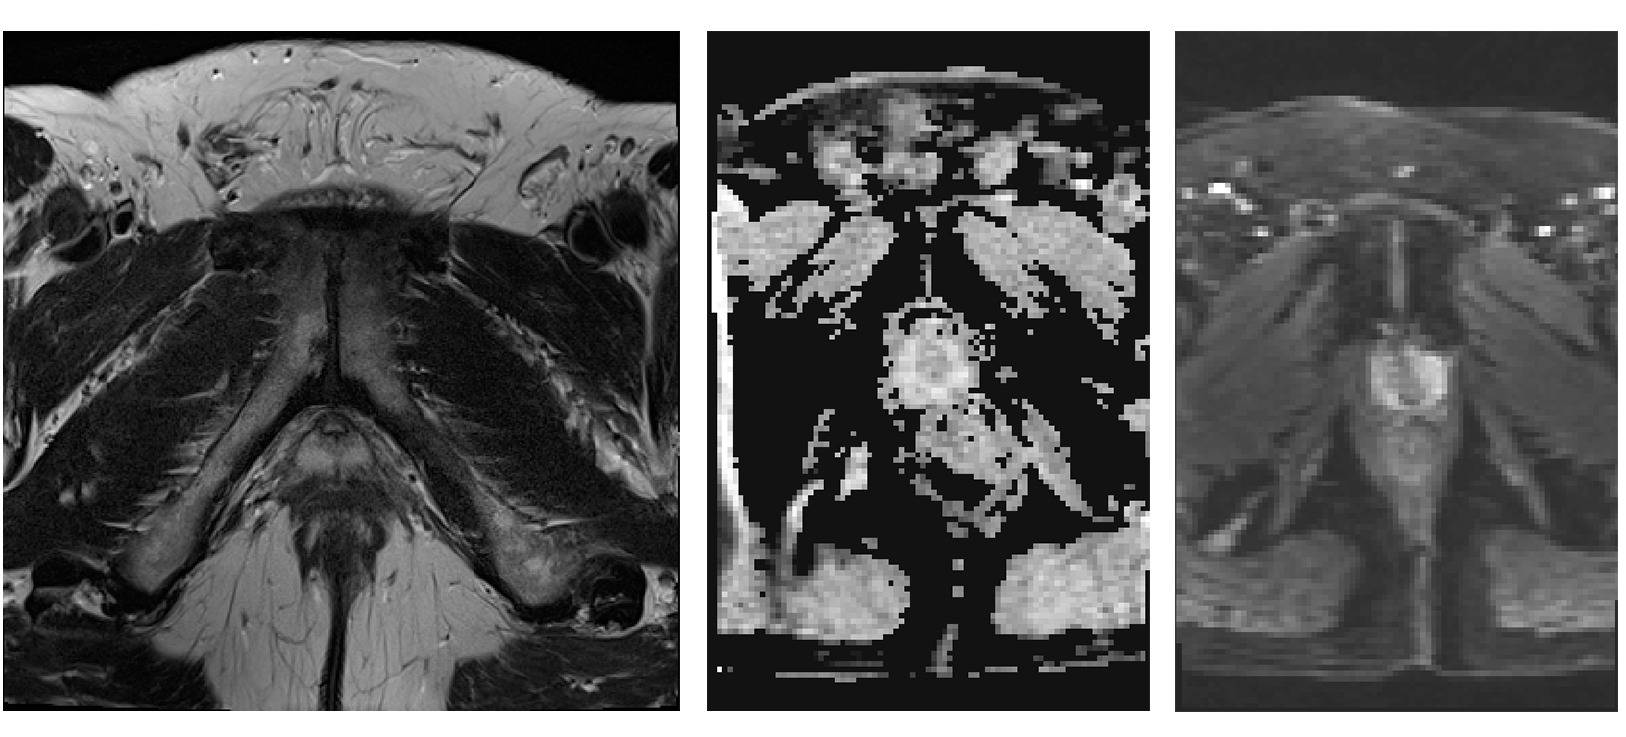
\includegraphics[width=1\textwidth, keepaspectratio=true]{./figures/PROSTATEx-t2-adc-dwi.png}
\caption{MRI sequences - PROSTATEx - From left to right: T2-weighted, ADC and DWI}
\label{fig:PROSTATEx-t2-adc-dwi}
\end{figure}


\section{DICOM file format}
\label{sec:DICOM}
\subsection{Origin}
\setlength{\marginparwidth}{3cm}\leavevmode \marginnote{\textbf{Cl{\'e}ment}}The acronym DICOM stands for Digital Imaging and Communications in Medicine. Before the 1980’s, images resulting from CT scans and MRIs were only decodable by machine manufacturers, while the medical community needed to export and share them for other tasks. For that reason, the ACR (American College of Radiology) and the NEMA (National Electrical Manufacturers Association) created a committee to build a standard. After two iterations with other names, DICOM was created in 1993. It standardized the representation of medical images and their transmission as it provided a network protocol built on top of TCP/IP.


\subsection{Data format}
\setlength{\marginparwidth}{3cm}\leavevmode \marginnote{\textbf{Cl{\'e}ment}}DICOM files can be viewed as containers of attributes, also called tags. The values of the pixels themselves are stored under the "Pixel Data" tag. Every single DICOM file usually represents a 2-dimensional image, which will form a 3-dimensional volume when put all together.

Other useful information such as the patient name and ID is directly stored within the DICOM files. This approach aims at linking each image to a specific person and event in order not to mix them up. Each DICOM file can be seen as part of a bigger dataset. 


\subsection{Processing images}
\setlength{\marginparwidth}{3cm}\leavevmode \marginnote{\textbf{Cl{\'e}ment}}When manipulating DICOM files, multiple details must be taken into account. 


\subsubsection{Order}
\setlength{\marginparwidth}{3cm}\leavevmode \marginnote{\textbf{Cl{\'e}ment}}First of all, the name of the files within datasets is a 6-digit number, from 000000 to the number of images minus one. However, this order does not match the real order of the images. In fact, the correct order is given by the "Instance Number" tag contained in the various files. Therefore, converted images must be sorted by instance number. 


\subsubsection{Data manipulation}
\label{sec:dicom_data_manipulation}
\setlength{\marginparwidth}{3cm}\leavevmode \marginnote{\textbf{Cl{\'e}ment}}CT and MRI machines, as well as monitors, differ from one manufacturer to the other and even from one model to the other. DICOM takes this problematic into account by providing specific tags that allow to display the exact same representation of the data, no matter the hardware used. Otherwise, physicians may struggle to detect anomalies because of color and exposition-related variations. 
Therefore, before displaying or converting an image to any format (such as PNG or NumPy array), pixel data must be normalized.

The procedure depends on the tags "Window Width" and "Window Center" (one always come with the other). These are used to represent a range of values corresponding to the pixel values in the data. For instance, a window center of 0 and a window width of 200 imply pixel values between -100 and 100.\\
If they are missing, a simple conversion is sufficient. The parameters used to convert the data are given by two tags: 
\begin{itemize}
	\item Bits allocated: the number of bits used to represent a single pixel (value: 1 or a multiple of 8)
	\item Samples per pixel: the number of channels for each pixel

\end{itemize}
\newpage
\noindent Examples: 
\begin{itemize}
\item 1 bit, 1 sample: black and white
\item 8 bits, 1 sample: grayscale
\item 8 bits, 3 samples: RGB
\item 16 bits, 1 sample: grayscale

\end{itemize} 

\noindent If they are included in the DICOM header, a linear transformation must be done to convert the stored representation of the pixels to the correct visualizable one. To achieve this, two steps are required: 

\begin{enumerate}
	\item \textbf{Apply the Hounsfield correction}\newline
	Hounsfield Units (HU) are used in CT images. It is a measure of radio-density, calibrated to distilled water and free air. Provided that the rescale slope and the rescale intercept are included in the DICOM header, the correction is applied thanks to the following formula:
\begin{equation}
	HU = m * P + b
\end{equation}
	where~$m$ is the rescale slope,~$P$ the pixel value, ~$b$ the rescale intercept.

	\item \textbf{Apply a linear transformation}\newline
	The result of the first operation then goes through a linear transformation based on the following conditions: 

\begin{equation}\label{eq:dicom1}
\textrm{if } (P \leq c - 0.5 - \frac{w-1}{2}) \textrm{, then }y = y_{min}
\end{equation}

\begin{equation}\label{eq:dicom2}
\textrm{else if } (P > c - 0.5 + \frac{w-1}{2}) \textrm{, then }y = y_{max}
\end{equation}

\begin{equation}\label{eq:dicom3}
\textrm{else } y = (\frac{P - (c - 0.5)}{w-1}) + 0.5) * (y_{max} - y_{min}) + y_{min}
\end{equation}

where~$c$ is the window center,~$w$ window width, ~$P$ the pixel input value, ~$y$ the pixel output value, ~$y_{min}$ the minimal value of the output range (usually 0), ~$y_{max}$ the maximal value of the output range (usually 255). Equations \ref{eq:dicom1}, \ref{eq:dicom2} and \ref{eq:dicom3} ensure that the pixel values are correctly distributed within the output range. 
\end{enumerate}


\section{NIfTI file format}
\subsection{Origin}
\setlength{\marginparwidth}{3cm}\leavevmode \marginnote{\textbf{Jobin}}The Neuroimaging Informatics Technology Initiative (NIfTI) file format is the successor of the ANALYZE file format. The main problem of the latter was a lack of information about orientation in space. Therefore, the interpretation of stored data could be problematic and inconsistent. For instance, there was a real confusion to determine the left and right sides of brain images. Hence, the NIfTI file format was defined to overcome this major issue.


\subsection{Data format}
\setlength{\marginparwidth}{3cm}\leavevmode \marginnote{\textbf{Jobin}}Unlike the ANALYZE format that used two files to store the metadata and the actual data, the NIfTI file format stores them in one single “.nii” file, but keeps this split between the real data and the header for compatibility. This has the advantage to facilitate the use of the data and avoid storing the data without the metadata. The NIfTI format can also be compressed/decompressed on the fly using the “deflate” algorithm. A. M. Winkler affirms that this is particularly useful as "it is very common for images to have large areas of solid background, or files describing masks and regions of interest containing just a few unique values that appear repeated many time"~\cite{52}.


\subsection{Overview of the header structure}
\setlength{\marginparwidth}{3cm}\leavevmode \marginnote{\textbf{Jobin}}With the goal of preserving the compatibility between the ANALYZE and the NIfTI formats, both headers have the same size of 348 bytes. A. M. Winkler confirms this fact by claiming that "some fields were reused, some were preserved, but ignored, and some were entirely overwritten"~\cite{52}. Details about the different fields contained in the header can be found in the references of the previous citation.


\section{RAW and MHD file formats}
\setlength{\marginparwidth}{3cm}\leavevmode \marginnote{\textbf{Cl{\'e}ment}}Some datasets use a combination of RAW and MHD files. The latter contain metainformation about their corresponding RAW file(s) which contain the data. In most cases, each MHD file points to a unique RAW file whose name is the same as the MHD file name. A single RAW file can be used to represent three-dimensional data, i.e. the combination of multiple two-dimensional images. Libraries such as \mbox{SimpleITK} in Python allow to manipulate RAW images in an easy way. 



\section{Visualization tools}
\setlength{\marginparwidth}{3cm}\leavevmode \marginnote{\textbf{Cl{\'e}ment}}Processing data manually increases the probability of making mistakes. For that matter, visualization tools relying on the same processing code as the ones used to generate training images were developed. Their primary goal is to compare our visual representation of an image to the one obtained in professional pieces of software. These tools are convenient to visualize a dataset easily. In some cases (especially RAW/MHD images), no free software capable of reading the files was available, which made the corresponding tool useful. 


\subsection{DICOM}
\setlength{\marginparwidth}{3cm}\leavevmode \marginnote{\textbf{Cl{\'e}ment}}Visualizing DICOM files is pretty straightforward since each file represents a single two-dimensional image. However, a lot of pixel transformations and normalizations have to be applied to obtain the desired result (see Section \ref{sec:dicom_data_manipulation}), which may be a source of errors. Our tool allows to display a single DICOM file as well as a sequence of files if the function is fed with a directory. Users can then scroll through the z-axis, displaying the next or previous slice.  Figure \ref{fig:visualize_lung_dcm} shows the visualization of a lung at three different z-axis coordinates. This allows the user to have a complete overview of the body part he wants to analyze.

\begin{figure}[!h]
\centering
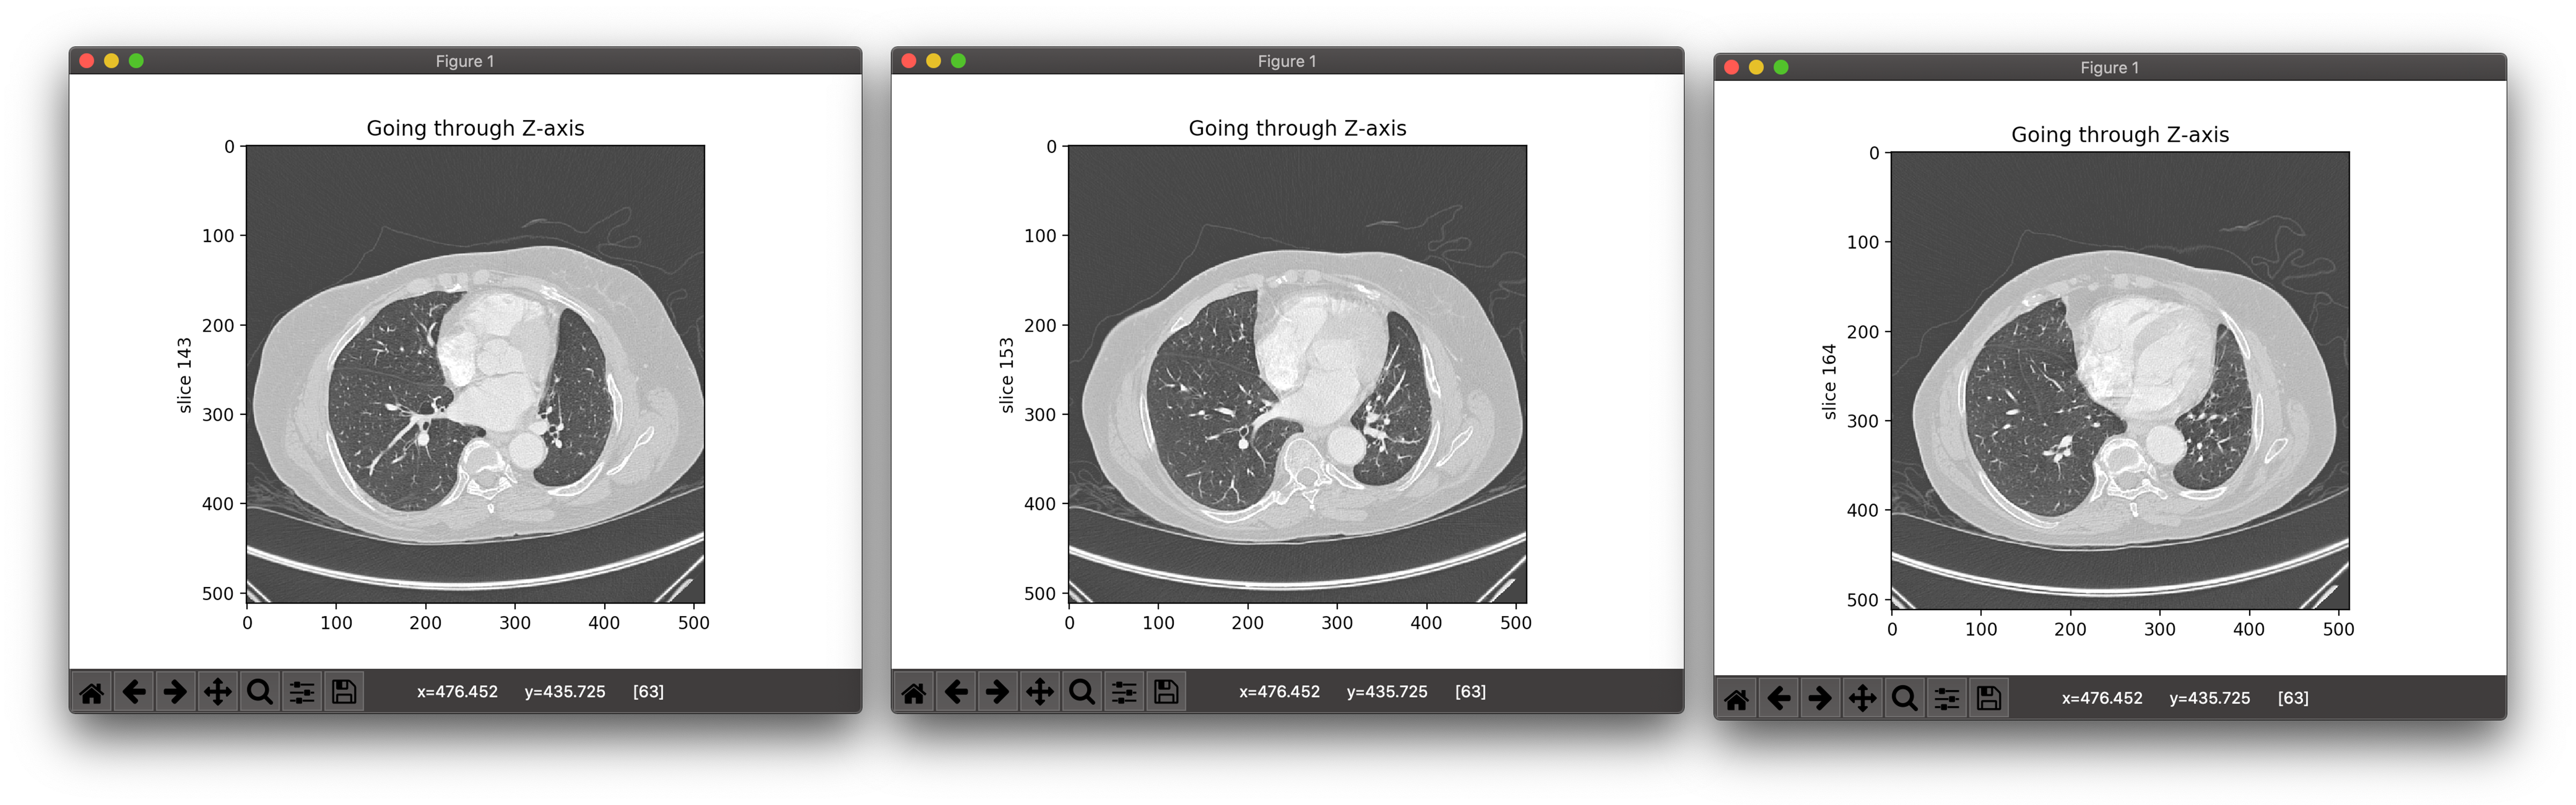
\includegraphics[width=\textwidth, keepaspectratio=true]{./figures/visualize_lung_dcm.png}
\caption{Visualization of a folder of DICOM files}
\label{fig:visualize_lung_dcm}
\end{figure}


\subsection{NIfTI}
\setlength{\marginparwidth}{3cm}\leavevmode \marginnote{\textbf{Cl{\'e}ment}}As a single NIfTI file can contain three- or four-dimensional data (the fourth dimension being time), our visualization tool takes this aspect into consideration by allowing to scroll through them: scrolling with the mouse goes through slices belonging to a specific timestamp over a specific axis, while the left and right arrows allow to jump to the same slice at another timestamp. When reaching the end of a timestamp with the mouse, the first slice of the next timestamp is displayed. Furthermore, the three-dimensionality implies that the volume is viewable from three different perspectives. For example, a three-dimensional brain volume can display it from the top of the head to the bottom, from one ear to the other and from the back of the head to the person's face. Therefore, the user can choose a specific axis to navigate through. If no axis is chosen, all three perspectives are shown one after the other.

\begin{figure}[!h]
\centering
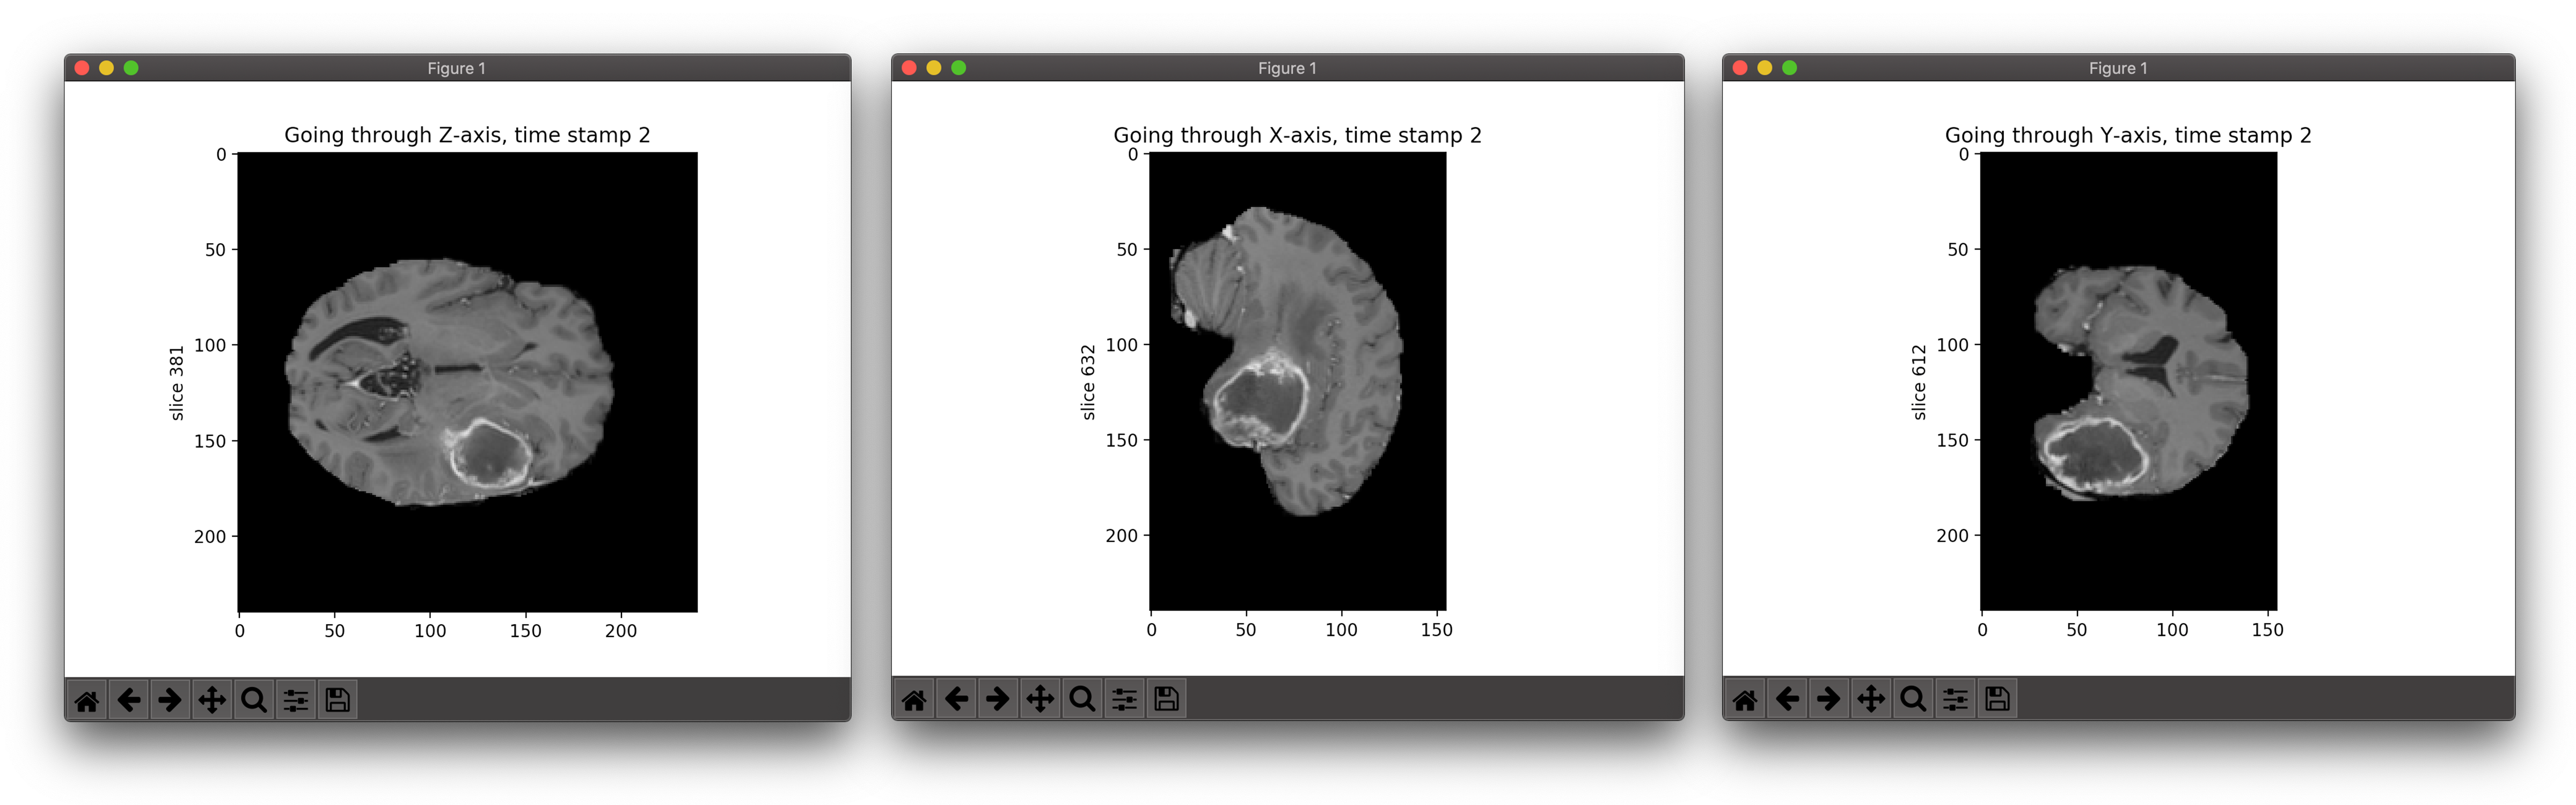
\includegraphics[width=\textwidth, keepaspectratio=true]{./figures/visualize_brain_nii.png}
\caption{Visualization of a four-dimensional NIfTI file}
\label{fig:visualize_brain_nii}
\end{figure}


\subsection{RAW}
\setlength{\marginparwidth}{3cm}\leavevmode \marginnote{\textbf{Cl{\'e}ment}}Medical RAW files are three-dimensional, which means that a single file contains a volume, i.e. a succession of 2D slices. Scrolling with the mouse goes through slices over a specific axis. Like the NIfTI file format, the user can profit from the three-dimensionality by displaying the body part under three different perspectives. This tool is particularly useful as no free software capable of handling these files is available. Photography-related programs such as Photoshop can open RAW pictures but not these three-dimensional ones. 

\begin{figure}[!h]
\centering
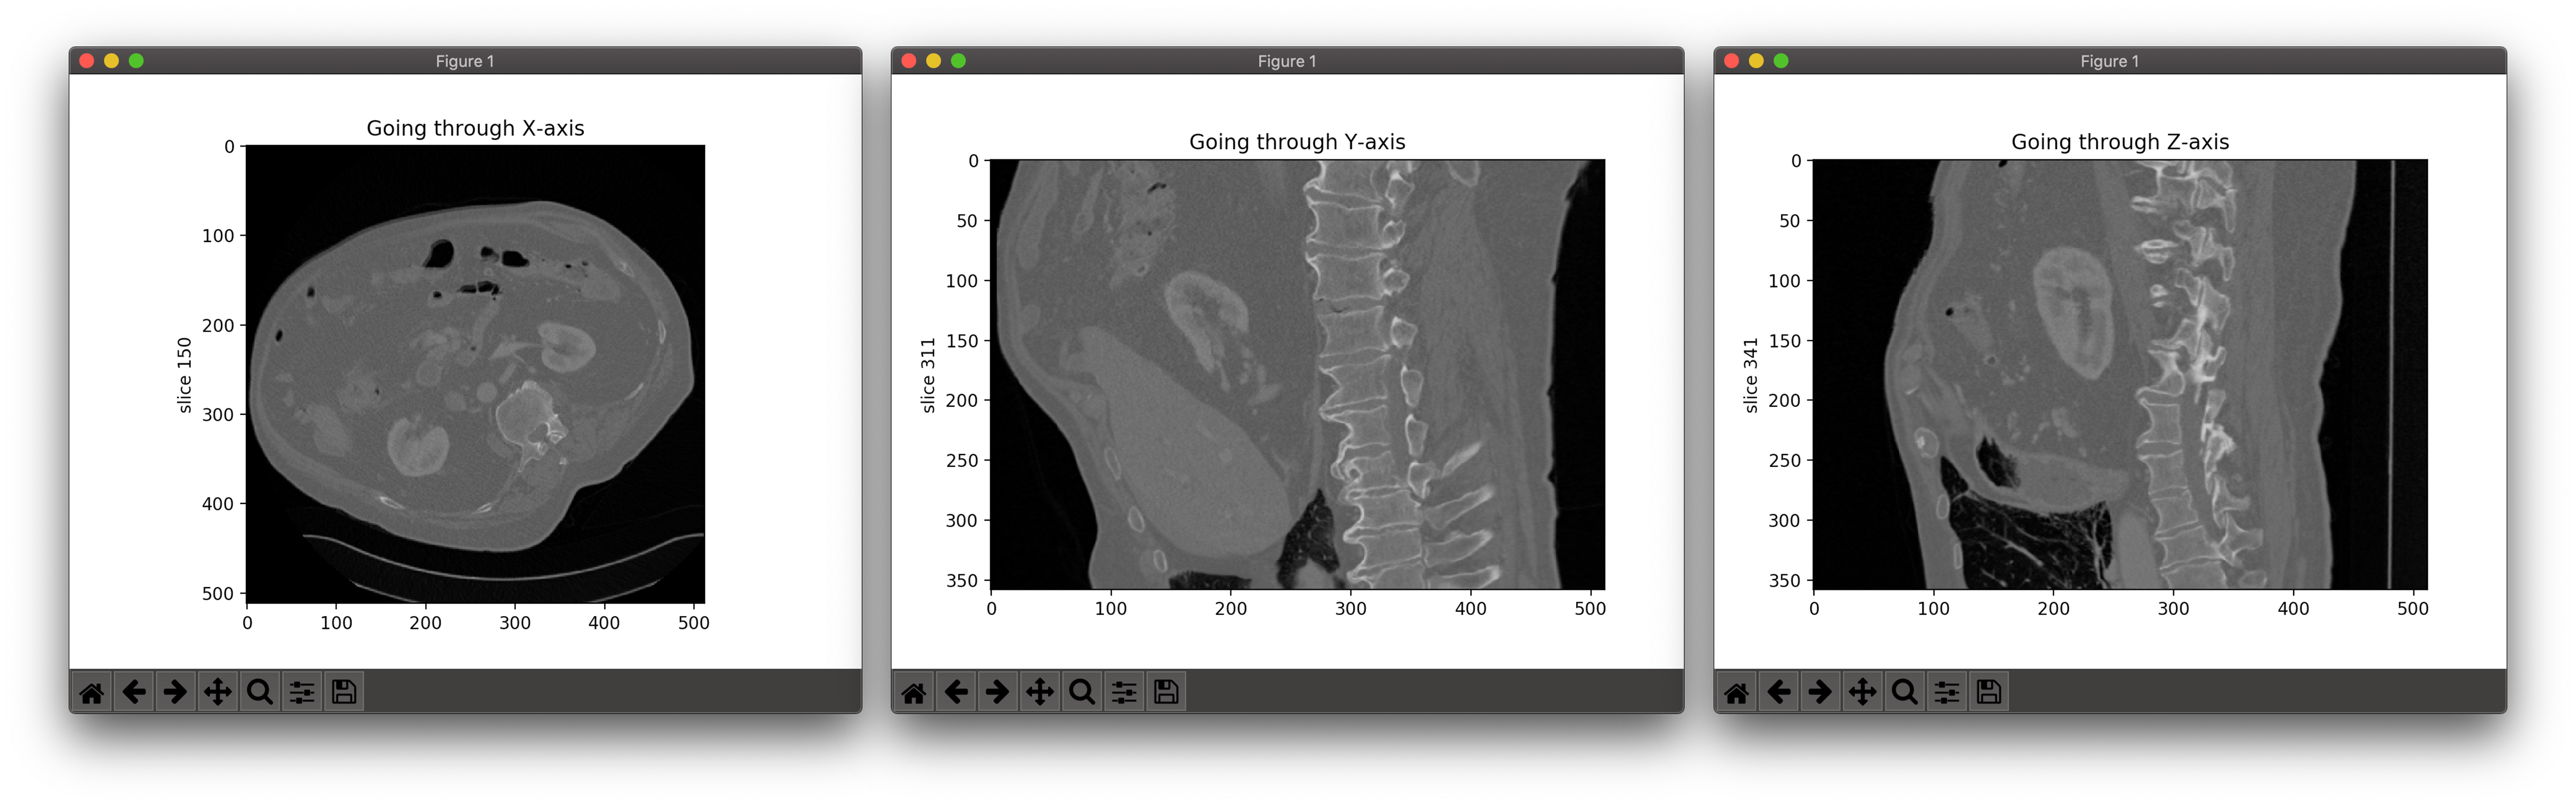
\includegraphics[width=\textwidth, keepaspectratio=true]{./figures/visualize_liver_raw.png}
\caption{Visualization of a three-dimensional RAW file}
\label{fig:visualize_liver_raw}
\end{figure}


\section{Conversion to PNG}
\setlength{\marginparwidth}{3cm}\leavevmode \marginnote{\textbf{Cl{\'e}ment}}In addition to the visualization tools, scripts allowing to convert medical files into PNG files were developed. The main one is called "anydatasettopng" and is the one to use to convert any file format to PNG as it makes use of the others. Given a root directory, it scans the latter and its subdirectories to find all DICOM, NIfTI and RAW/MHD files. Then, each file is converted to PNG and saved into the same directory as the one it came from. This script allows to keep an easily accessible visual representation of medical files without having to rely on a specific piece of software to display them. Finally, it also played the role of a debugging tool since the conversion techniques are the same as the ones used further in this work. 


\subsection{8-bit conversion}
\setlength{\marginparwidth}{3cm}\leavevmode \marginnote{\textbf{Cl{\'e}ment}}Medical data is often represented over 16 bits. However, exporting images to PNG requires 8-bit images. To transpose a 16-bit image to an 8-bit one, the procedure described by algorithm \ref{alg:16_to_8_bits_conversion} was applied. 

\begin{algorithm}
    \caption{16 to 8 bits conversion}
    \label{alg:16_to_8_bits_conversion}
    \begin{algorithmic}[1] % The number tells where the line numbering should start
        \Procedure{16\_to\_8\_bits\_conversion}{$pixel\_array$}
        		\State{$Pixel_{min} \gets$ minimal pixel value in $pixel\_array$}
        		\State{$Pixel_{max} \gets$ maximal pixel value in $pixel\_array$}
        		\For{$pixel\_value$ in $pixel\_array$}
        			\State $pixel\_value \gets \frac{(pixel\_value - Pixel_{min}) * 255.0}{Pixel_{max} - Pixel_{min}}$
        		\EndFor
        		\State Modify object type to 8 bits
        		\State Export $pixel\_array$ as PNG
        \EndProcedure
    \end{algorithmic}
\end{algorithm}